%declaration package
\documentclass[12pt,a4paper]{article}
\usepackage[french]{babel} 
\usepackage[utf8]{inputenc}
\usepackage[T1]{fontenc}
\usepackage{amsmath,amsfonts,amssymb}
\usepackage{makeidx}
\usepackage{graphicx}
\usepackage{wrapfig}
\usepackage{xcolor}
\usepackage{listings}
\usepackage{float}
\usepackage[top=2cm, bottom=2cm, left=2cm, right=2cm]{geometry}
\usepackage{titlesec}
\usepackage{url}
\usepackage{subfigure}
\usepackage{textcomp}
\usepackage{hyperref}

\definecolor{darkWhite}{rgb}{0.94,0.94,0.94}

\lstset{
  aboveskip=3mm,
  belowskip=-2mm,
  backgroundcolor=\color{darkWhite},
  basicstyle=\footnotesize,
  breakatwhitespace=false,
  breaklines=true,
  captionpos=b,
  commentstyle=\color{red},
  deletekeywords={...},
  escapeinside={\%*}{*)},
  extendedchars=true,
  framexleftmargin=16pt,
  framextopmargin=3pt,
  framexbottommargin=6pt,
  frame=tb,
  keepspaces=true,
  keywordstyle=\color{blue},
  language=c,
  literate=
  {²}{{\textsuperscript{2}}}1
  {⁴}{{\textsuperscript{4}}}1
  {⁶}{{\textsuperscript{6}}}1
  {⁸}{{\textsuperscript{8}}}1
  {€}{{\euro{}}}1
  {é}{{\'e}}1
  {è}{{\`{e}}}1
  {ê}{{\^{e}}}1
  {ë}{{\¨{e}}}1
  {É}{{\'{E}}}1
  {Ê}{{\^{E}}}1
  {û}{{\^{u}}}1
  {ù}{{\`{u}}}1
  {â}{{\^{a}}}1
  {à}{{\`{a}}}1
  {á}{{\'{a}}}1
  {ã}{{\~{a}}}1
  {Á}{{\'{A}}}1
  {Â}{{\^{A}}}1
  {Ã}{{\~{A}}}1
  {ç}{{\c{c}}}1
  {Ç}{{\c{C}}}1
  {õ}{{\~{o}}}1
  {ó}{{\'{o}}}1
  {ô}{{\^{o}}}1
  {Õ}{{\~{O}}}1
  {Ó}{{\'{O}}}1
  {Ô}{{\^{O}}}1
  {î}{{\^{i}}}1
  {Î}{{\^{I}}}1
  {í}{{\'{i}}}1
  {Í}{{\~{Í}}}1,
  morekeywords={*,...},
  numbers=left,
  numbersep=10pt,
  numberstyle=\tiny\color{black},
  rulecolor=\color{black},
  showspaces=false,
  showstringspaces=false,
  showtabs=false,
  stepnumber=1,
  stringstyle=\color{gray},
  tabsize=4,
  title=\lstname,
}

\begin{document}

%page de garde

\begin{titlepage}
\newcommand{\HRule}{\rule{\linewidth}{0.1mm}}
\center


\includegraphics[scale=0.4]{logo.png} \\[0.2cm]

\includegraphics[scale=0.7]{CHPS_logo.png} 
\\[1.2cm]
\HRule \\[0.4cm]
{ \huge \bfseries Projet de Programmation Numérique sur Machine Parallèle \\ "TASKIFICATION"
  \\[0.15cm] }
\HRule 

\href{https://github.com/Taskification/Taskification}{\color{blue}Dépôt Git} 
\\[1.5cm]
Encadré par : \textbf {Jean-Baptiste Besnard } \\ [1cm]

\textbf{Réalisé par :} \\ [0.3cm] Sofiane BOUZAHER  \\ Asma  KREDDIA \\ Karim SMAIL \\ Atef DORAI 
\\[0.5cm]M1CHPS \\[5cm]
\today \\ [1cm]
\end{titlepage}

%remerciement

\vspace*{\stretch{1}}
\begin{center}
	\begin{minipage}{13cm}


\section*{ \huge \bfseries \center Remerciements}
Nous souhaitons avant tout remercier notre encadrant de projet, Jean-Baptiste BESNARD, pour le temps qu’il a consacré à nous apporter les outils méthodologiques indispensables à la conduite de cette recherche. Son exigence nous a grandement stimulé.

L’enseignement de qualité dispensé par le Master « CHPS » a également su nourrir nos réflexions et a représenté une profonde satisfaction intellectuelle, un grand merci donc aux enseignants.

	\end{minipage}
\end{center}
\vspace*{\stretch{1}}





\pagebreak
%sommmaire
\listoffigures

%\renewcommand*\contentsname{Sommaire}
\tableofcontents

\pagebreak

%rapport
\section{Titre du Sujet}

Analyse Statique Pour la Classification des Procédures Candidate à la « Taskification »

\section{Introduction}

Comme on a déjà vu précédemment au premier semestre l'objectif de notre projet est la mise en place d’un plugin dans le compilateur CLANG (LLVM) pour identifier les appels de fonctions candidats à la « taskification » (fonctions pures), l'objectif sous-jacent est l'identification du potentiel de parallélisation automatique du code en trouvant les fonctions pures et ensuite en les insérant dynamiquement dans des appels de fonctions parallèles via des Remote Procesure Call (RPC).

Pour ce faire, il faudra: 


\begin{itemize}
	\item Mettre en place la structure de base d’un plugin clang.
	\item Définir ce qui distingue les fonctions candidates à identifier.
	\item Implémenter ce support dans le plugin;
	\item Le valider sur un cas de parallélisme producteur / consommateur.
\end{itemize}

\subsection{Mots Clefs}

Bibliothèque Clang LLVM, RPC,AST,Makefile ,PLugin


\subsection{Description Générale}

Les architecture hybrides convergées à venir posent la question des modèles de programmation. En effet MPI depuis l’avènement des architectures many-core a dû être combiné avec du paralslélisme intra-noeud en OpenMP (MPI + X). Le mélange de ces modèles se traduit nécessairement par une complexité accrue de l’expression des codes de calcul. Dans ce travail nous proposons de prendre cette tendance à contre-pied en posant la question de l’expression de tâche de calcul en pur MPI. Les étudiants se verront fournir une implémentation de Remote Procedure Calls (RPC) implémentés en MPI, le but du travail est de détecter quelles fonctions sont éligibles à la sémantique RPC statiquement lors de la phase de compilation (c.a.d. les fonction dites « pures »: indépendantes du tas, des TLS, etc …). Le travail visera le compilateur LLVM dans lequel une passe sera rajoutée pour lister l’ensemble des fonctions éligibles à la sémantique RPC. Pour exemple, une implémentation d’un algorithme de cassage de mot de passe en MPI sera fournie avec pour but sa conversion en RPC producteur/consommateur (github.com/besnardjb/MPI\_Brute/) avec l’outil.

 \subsection{Objectif Général}

Le but d'un programme est d'exécuter  une tâche. Pour réaliser celle-ci, on donne à l'ordinateur une liste d'instructions qu'il va effectuer. Il existe plusieurs manières de traiter ces instructions, parmi ces manières, on trouve la programmation parallèle.

\paragraph{}\textbf{Pourquoi le parallélisme ?}

 L’exécution de  certaines fonctions d'un programme de manière parallèle, nous permet un gain de temps d'exécution du programme, ce qui veut dire rendre le programme plus performant qu'avant, mais ceci n'est pas applicable à tous les algorithmes. Dans ce projet nous cherchons donc à développer une méthode automatisée pour localiser les portions de programme qui sont candidates à la parallélisation automatique.

\section{Résumé des Travaux du Premier Semestre}

Précédemment au projet effectué en semestre 1 on s'est projeté sur plusieurs points : 

\subsection{Fonctions pures/impures}
On a commencé à définir ce qu'est une fonction pure et une fonction impure car les deux sont des fonctions candidates à la "Taskification" .\\
On a défini une fonction pure comme étant une fonction qui ne dépend pas et ne modifie pas l'état de variable qui n'est pas à ça portée ,son principal avantage est qu'elle est prédictible c'est à dire facile à tester  et on a cité quelques exemples sur les fonctions pures comme la fonction max,min et floor .\\
Pour les fonctions impures ce sont des fonctions a effets de bord c'est à dire elles renvoient des valeurs différentes à chaque appel . Une fonction peut être impure à cause de plusieurs raisons :

    \begin{itemize}
    \item la variation de la valeur de retour avec une variable non locale.
    \item la variation de la valeur de retour avec un argument mutable de type référence
    \item la variation de la valeur de retour avec un flux d’entrée.
    \item la mutation d’une variable statique locale.
    \item la mutation d’un argument mutable de type référence.
    \item la mutation d’un flux de sortie.
\end{itemize}

\subsection{Présentation de CLANG \cite{clangllvm}  }

On a commencé par définir l'infrastructure clang - LLVM  comme étant une collection de compilateurs modulaires ,réutilisables et de technologies de chaîne d’outils. Pour mieux comprendre l’ensemble des étapes de compilation par cette infrastructure,on a défini :
    \begin{itemize}

    \item le Frontend : qui est le premier bloc de tout compilateur son objectif est de voir si le programme est syntaxiquement et sémantiquement correct puis le traduire vers une présentation intermédiaire(IR) pour simplifier le travail des autres blocs.
    \item Les Passes : qui sont en charge d'analyser et/ou de transformer l'IR en optimisant certaines choses .l'objectif est de maximiser les performances du code.
    \item le backend : est en charge de transformer l'IR vers du code machine afin d'intervenir aux différents niveaux de la chaine de compilation .
     \end{itemize}
 On a défini aussi CLANG,OPT,LLC,LLVM-AS/LLVM-DIS et LLI comme des outils qui participent a la compilation et l'execution.



\subsection{Generalité sur l'AST}

Au cours de la compilation avec Clang on passe par 3 étapes: Frontend qui prend en charge la partie analyse, ie la décomposition du code source en morceaux selon une structure grammaticale, le résultat sera transformé  dans un target program par le Backend,cette étape est appelée synthèse, tout en passant par une étape intermédiaire d'optimisation entre le Frontend et le Backend.\cite{Devlieghere}\\ Donc l’AST est une représentation structurée de la syntaxe du code que l’on analyse. L’AST est en fait une structure en C++ assez complexe de classes avec héritages.\\


 On a aussi vu plusieurs définitions utiles comme celles de l'analyse statique , l'analyse dynamique, la compilation , la mémoire partagée et la mémoire distribuée .


\section{Concepts Clef}

\subsection{Objectif du Projet}

Le but est la mise en place d’un plugin dans le compilateur CLANG (LLVM) pour identifier les appels de fonctions candidats à la « taskification » (fonction pure) ,pour ce faire, il faudra mettre en place la structure de base d’un plugin clang ,définir ce qui distingue les fonctions candidates à identifier , et enfin implémenter ce support dans le plugin et  Le valider sur un cas de parallélisme producteur / consommateur.

\subsection{Définitions Utiles} 
	
\textbf{ LLVM (Low Level Virtual Machine):} est une infrastructure de compilateur conçue pour l'optimisation du code à la compilation (c’est une infrastructure qui ne contient pas des outils nécessaires pour compiler du code source C ou C++ mais uniquement des outils d’optimisations et de génération de codes machine à partir d’un format intermédiaire).\cite{clangllvm}
              
\textbf{CLANG-LLVM :} la structure générale de cette infrastructure à l’échelle microscopique est constitué d’une façon similaire à tout compilateur moderne .\cite{clangllvm}


\textbf{ MPI:} Message Passing interface, est une norme conçue pour le passage de messages entre ordinateurs distants ou dans un ordinateur multiprocesseur ( donc c’est un moyen de transfert de message créer pour obtenir de meilleures performances), Elle est devenue un standard de communication pour des nœuds exécutant des programmes parallèles sur des systèmes à mémoire distribuée. Elle définit une bibliothèque de fonctions, utilisable avec les langages C, C++ et Fortran.\cite{wiki}


\textbf{ La parallélisation automatique :} c’est l’un des stages de compilation d’un programme au niveau de lequel le code source est transformé  en un exécutable parallélisé pour ordinateur à un multiprocesseur symétrique dont le but de simplifier et de réduire la durée de développement des programmes parallèles.\cite{wiki}

\textbf{ Un multiprocesseur symétrique ( ou symmetric shared memory multiprocessor -SMP): } 
le but principal de cette architecture parallèle  est de multiplier les processeurs identiques sur un ordinateur, afin d’améliorer  la puissance de calcul.\cite{wiki}

\textbf{ Remonte Procédure Calls (RPC) : } définie comme étant un moyen de communication qui permet de faire appeler des procédures sur un ordinateur a distance en utilisant un serveur d'application.\cite{wiki}

\textbf{Plugin Clang :} Le compilateur Clang peut être étendu à l'aide d'un plugin qui permet d'exécuter des actions supplémentaires déjà définies par l'utilisateur au moment de la compilation\cite{ClangTeam}, c'est a dire qu'il peut fournir des avertissements et des erreurs de compilation en plus, ou effectuer des modifications de code source.\cite{clang}

\textbf{Makefile :} Les Makefiles sont des fichiers, généralement appelés makefile avec m minuscule ou Makefile avec m majuscule ,ils sont utilisés par le programme make qui est un logiciel de construction automatique ,pour exécuter un ensemble d'actions.\cite{makefile}
\section{Description de notre Plugin:}

\subsection{Clang plugin:}

Rappelons que le plugin est une librairie dynamique chargée par le compilateur au moment de l’exécution d’un code source.
Notre plugin «impurewarnings»  permet de détecter le type de fonctions dans un code source, pures ou impures, lors de la compilation. \\
En chargeant notre plugin lors d’une nouvelle compilation, nous attendons un WARNING pour chaque fonction impure  et une liste contenant toutes les fonctions impures.\\

Pour qu'un plugin fonctionne parfaitement, il doit contenir: 
\begin{itemize}
    \item un code source en cpp basé sur 3 classes:\\
	 Class \textbf{PluginASTAction}.\\
	 Class  \textbf{ASTConsumer.}\\
	 Class \textbf{RecursiveASTVisitor}.
\item un Makefile  pour générer la bibliothèque dynamique et exécute le plugin.
\end{itemize}

\subsection{Description du code source de plugin:} 

Ci-dessous les entêtes standard qui appartient à la documentation clang et qui sont requis pour le code: 

\begin{figure}[H]
\centering
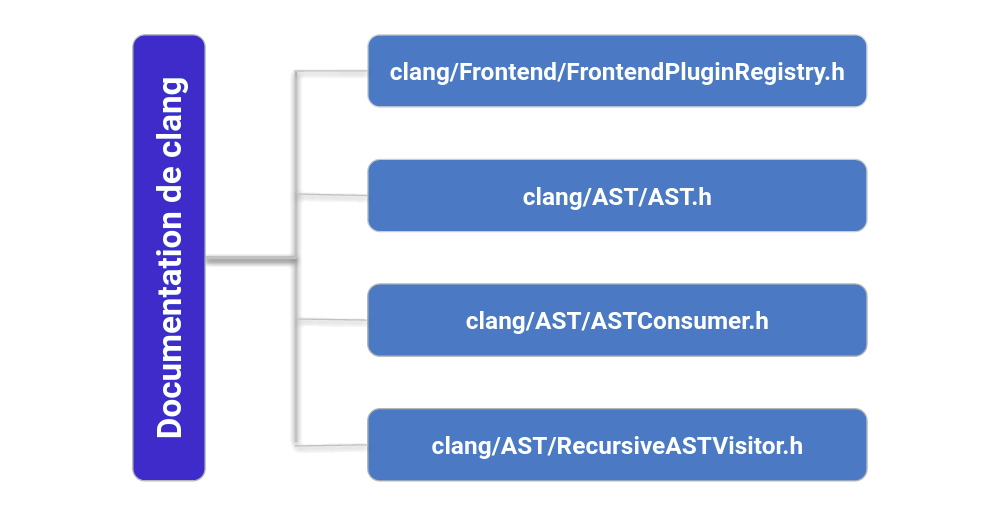
\includegraphics[scale=0.5]{headerss.png} 
\caption[Les Entêtes]{Les Entêtes utilisés} 
\end{figure}


\textbf{ASTAction:}

la classe PluginASTAction personnalisée est une classe de base abstraite à utiliser pour  le class ASTConsumer. Il s’agit d’un point d'entrée à partir duquel nous pouvons invoquer notre ASTConsumer.\\
\begin{figure}[H]
\centering
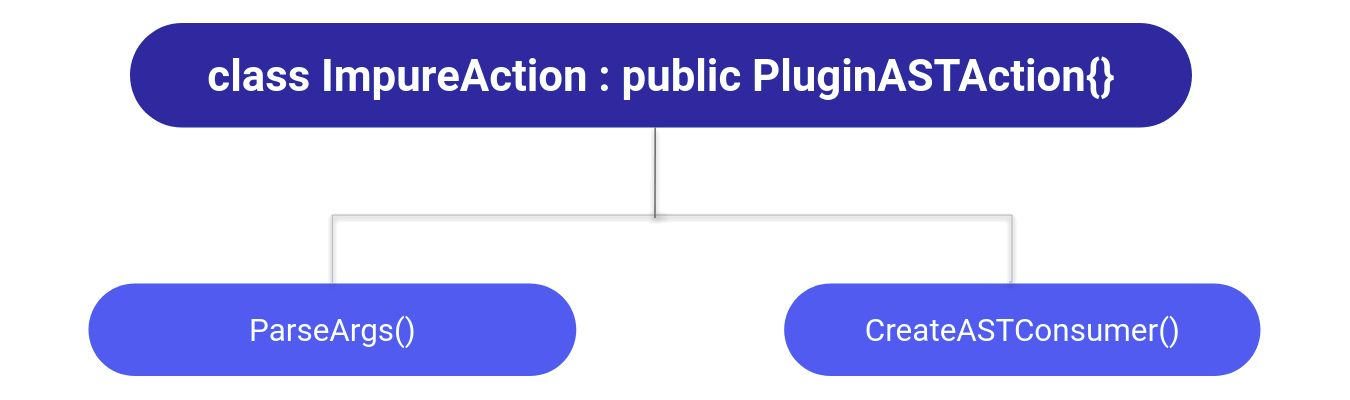
\includegraphics[scale=0.75]{action-1.png} 
\caption[ASTAction]{ASTAction} 
\end{figure}

Cette classe contient deux fonctions:

\begin{itemize}
    \item \textbf{CreateASTConsumer:} cette fonction est appelée automatiquement par Clang  lorsqu'on charge le plugin lors de la compilation.
	\item \textbf{ ParseArgs:} cette fonction est indispensable pour analyser les arguments de «command line ».
\end{itemize}

\textbf{ASTConsumer:} 

La tâche principale de l’ASTConsumer est de parcourir  l'AST généré par l'analyseur du Clang, afin que notre code soit appelé lorsqu'un certain type d'élément AST a été analysé.\\
Dans notre class ImpureExprConsumer vous trouverez 3 fonctions:
\begin{figure}[H]
\centering
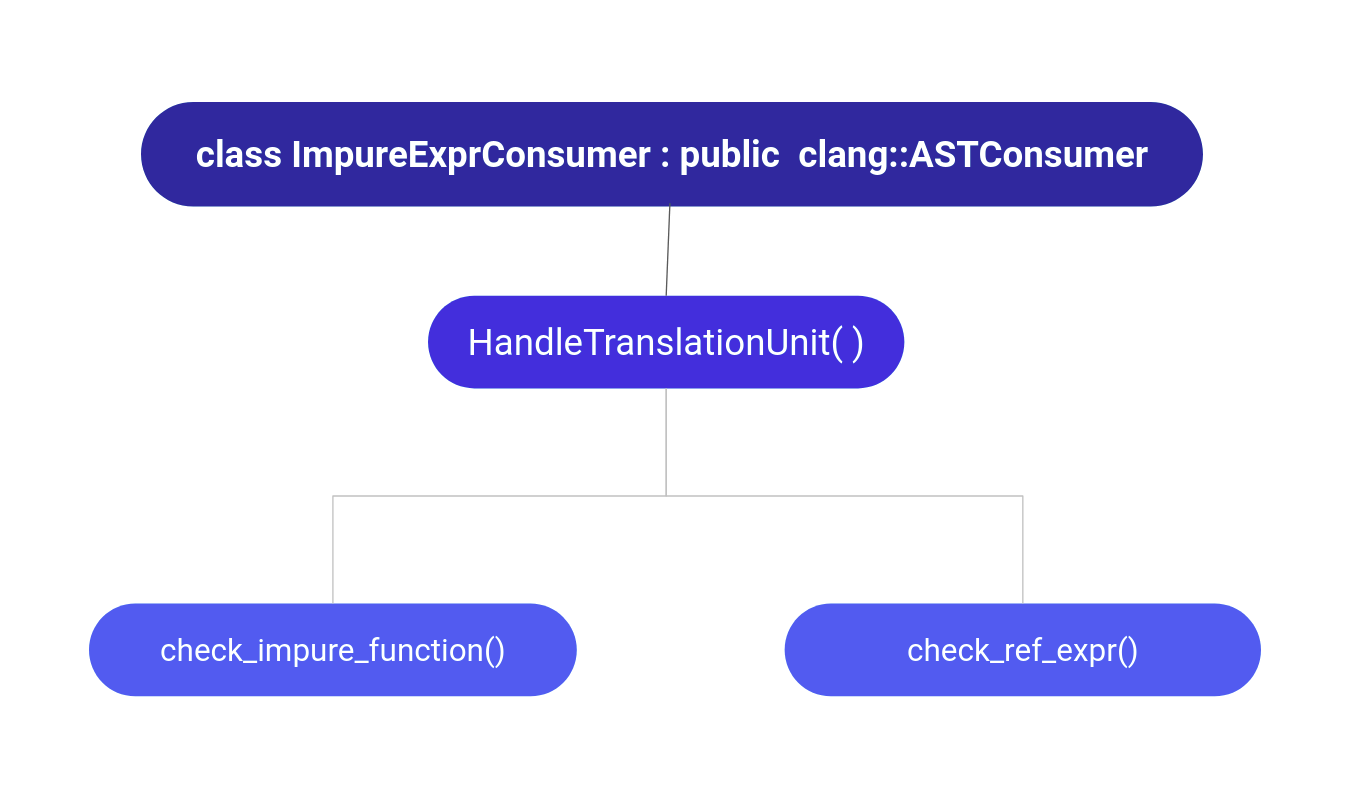
\includegraphics[scale=0.75]{cons-3.png} 
\caption[ASTConsumer]{ASTConsumer} 
\end{figure}

\begin{itemize}
    \item \textbf{HandleTranslationUnit :}cette fonction appartient a la documentation officielle du clang, et qui sera appelée chaque fois qu’on parcoure un nouvel ensemble de déclarations de niveau supérieur comme une variable globale ou une  définition de fonction.
\end{itemize}

\textbf{Remarque}: HandleTranslationUnit est appelée qu'après la fin de l’analyse complète du fichier source, donc on a besoin d’ASTContext qui nous permet de garder la représentation de l’AST après l’analyse, ASTContext  est utilisé pour obtenir le TranslationUnitDecl , qui représente l'intégralité du fichier source sous forme d’un seul Decl. \\

\begin{itemize}
\item A chaque fois qu’on traverse une nouvelle déclaration de fonction (détection d’un FunctionDecl dans l’AST), la fonction \textbf{check\_impure\_function}  sera appelé.
\item A chaque fois qu’on traverse une nouvelle déclaration d’une variable (détection d’un VarDecl dans l’AST), on l’affiche .
 \item A chaque fois qu’on traverse un appel vers une fonction extérieur ou une variable globale (détection d’un DeclRefExpr dans l’AST) la fonction \textbf{ check\_ref\_expr} sera appelé.
 \end{itemize}

\textbf{check\_impure\_function:}
 Cette fonction affiche le corps de la fonction et en même temps vérifie si la fonction fait un appel vers une autre fonction ou non, dans le cas ou c’est vrai un WARNING sera affiché. 

\textbf{check\_ref\_expr:}	
 Cette fonction vérifie si on fait un appel vers une variable globale ou non, dans le cas ou c’est vrai un WARNING sera affiché. 
\begin{itemize}
\item Chaque fonction dans cette classe associe à un RecursiveASTVisitor, comme nous allons l’expliquer ci-dessous.
\end{itemize}

\textbf{RecursiveASTVisitor:}

À l’aide de deux classes précédentes on a préparé l’infrastructure de notre plugin,  en parcourant  la documentation officielle de RecursiveASTVisitor. On trouve de nombreuses fonctions  telle que :  VisitFunctionDecl , VisitStmt,... qui nous  permettent de visiter tous les types de nœud dans l’ AST.

Un plugin ne doit jamais appeler une fonction de visite de façon directe ,il faut toujours passer par une fonction qui appartient a  la classe ASTConsumer qui appellera la fonction de visite correcte en arrière-plan, et chaque fonction de visite doit retourner ‘true’ pour continuer a parcourir l’AST  . 

Notre objectif est de détecter toutes les fonctions impures du coup on a besoin de visiter toutes les variables globales à l’aide  de  VisitVarDecl et toutes les fonctions à l’aide de VisitFunctionDecl , encore plus loin on doit visiter et parcourir les contenus de chaque fonction pour vérifier si on a un appel vers l’extérieur c’est-à -dire vers une variable globale ou vers une autre fonction différente de la fonction elle-même , on peut visiter tous les appels à l’aide de VisitDeclRefExpr.

Si on résume, cette  classe contient 3 fonctions ,et qui sont: 
\begin{figure}[H]
\centering
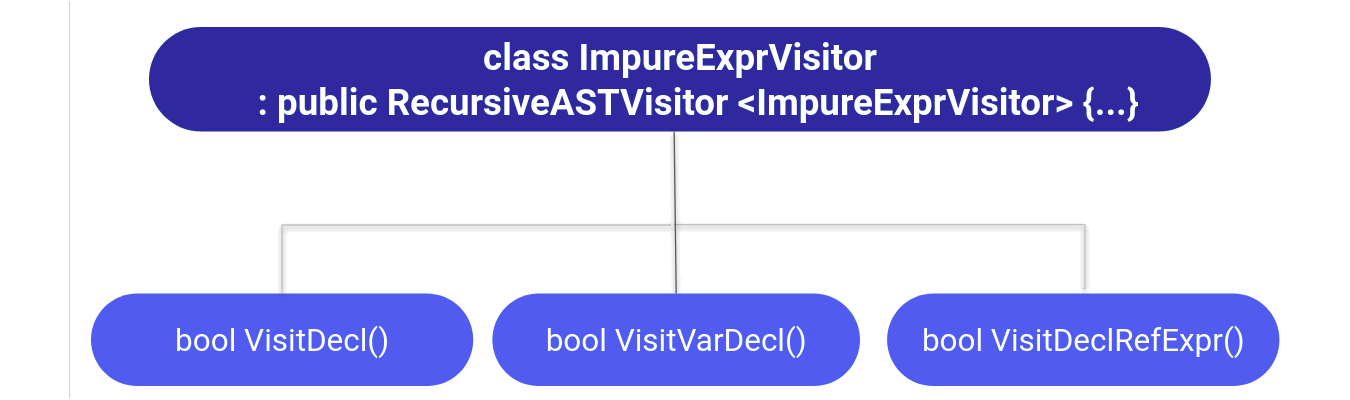
\includegraphics[scale=0.75]{vis-1.png} 
\caption[ASTVisitor]{ASTVisitor} 
\end{figure} 

\begin{itemize}
\item  \textbf{VisitDecl:} qui nous permet de visiter tous les Decl ,et vérifier à l’aide de \textbf{ dyn\_cast} si le decl est un FunctionDecl ou non, afin de stocker toutes les fonctions dans  un vector.
\item \textbf{VisitVarDecl:} pour chaque VarDecl elle vérifie si la variable déclarée est globale ou pas , et la stocker dans un vector .
\item \textbf{VisitDeclRefExpr:} cette fonction est appelée pour chaque DeclrefExpr dans l’AST et le stocker dans un vector .
\end{itemize}

\subsection{ Exécution du Plugin:}

\begin{itemize}
    \item \textbf{load:}
Pour exécuter un plugin, la librairie dynamique contenant le registre de plugin doit être chargée via la commande -load, ainsi on demande à clang de charger la librairie impureplugin.so et d'utiliser le plugin nommé  impurewarnings.
\item \textbf{ Xclang:}
En clang, l'argument Xclang indique que lors de la compilation ce paramètre permet de transférer les arguments du driver vers le compilateur.
\end{itemize}
\subsection{Teste de fiabilité du Plugin}
On teste notre plugin à partir du fichier source qui représente un exemple d'application de notre plugin : 

\begin{lstlisting}
#include <stdio.h>

int global_variable = 99;

int pure(void)
{
	return 5;
}

int impure()
{	
	global_variable = 9;
	printf("LL\n");
	return 0;
}

int main(int arcg, char ** argv)
{
	pure();
	impure();
	return 0;
}
\end{lstlisting}

Et on obtient l'AST généré par notre plugin ci-dessous :

\begin{figure}[H]
\centering
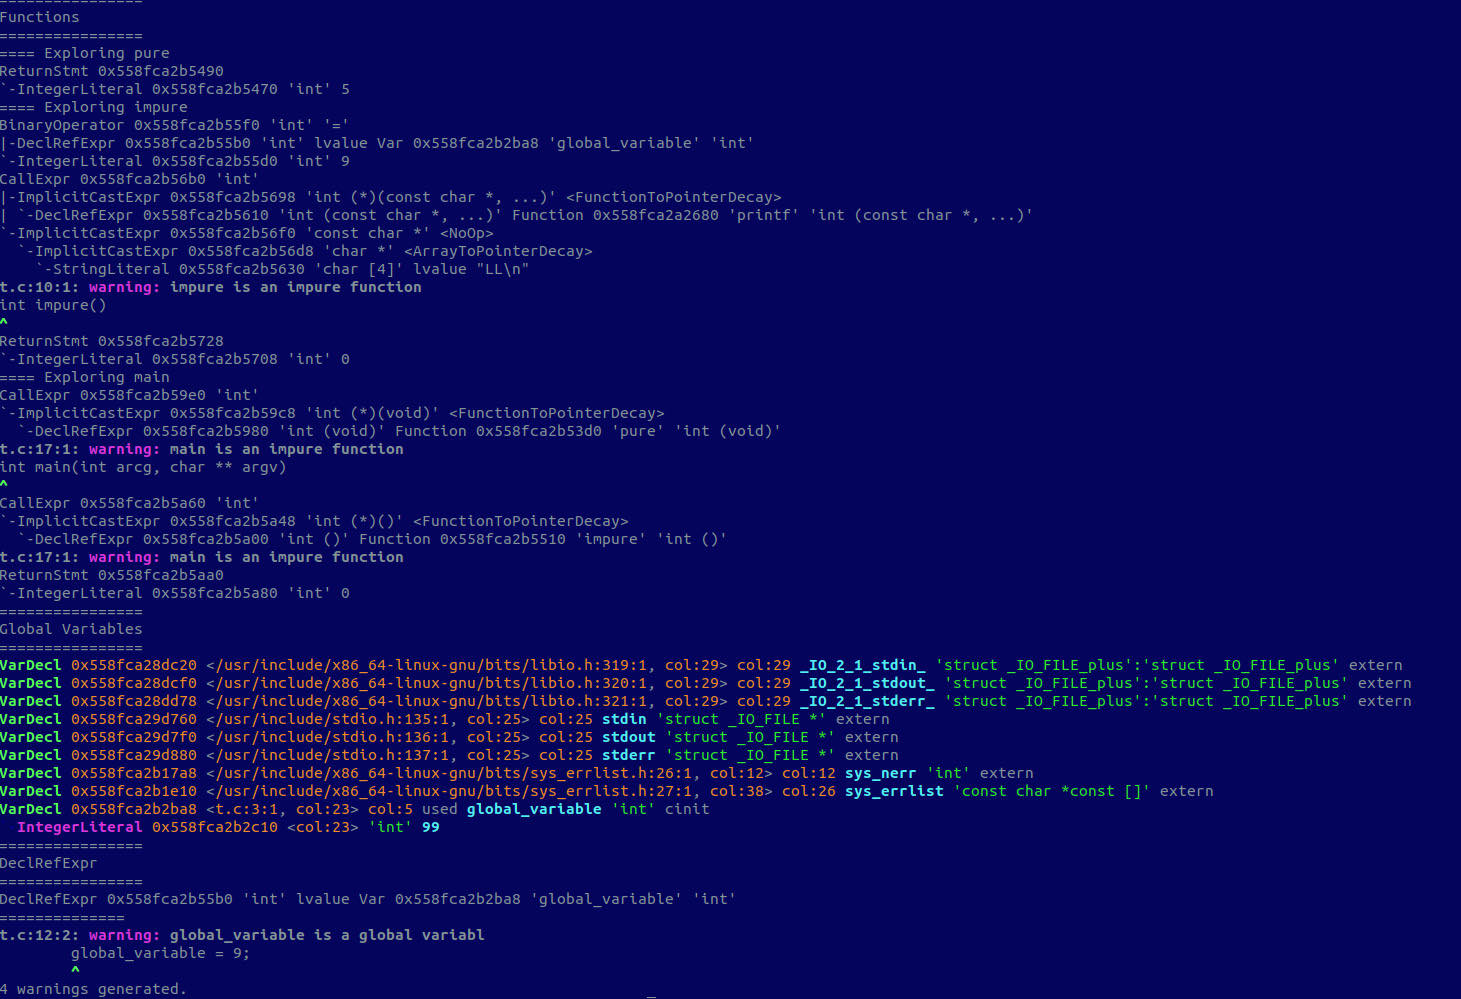
\includegraphics[scale=0.35]{AST.jpg}
\caption[Résultats]{Résultats} 
\end{figure}

Notre plugin détecte les fonctions pures, qui sont des fonctions indépendantes aux autres fonctions, c'est-à-dire leur résultat ne dépend pas des résultats des autres fonctions (ne dépend qu'elle-même car elle répond toujours la même chose pour les mêm
\section{Parallélisation via RPC }

\subsection{Remote Procédure Calls (RPC) principes :}
Le principe est de lancer n processus qui peuvent s'exécuter en n coeur différents et de permettre aux différents processus d'échanger des traitements en procédant à des appels de fonctions à distance. On a donc une fonction qui permet d'appeler les fonctions à distance (c'est ce qu'on appelle RPC, Remote Procedure Call), il faut juste appeler MPIX\_Offload qui prend en paramètres :

\begin{itemize}
\item Les paramètres (buffers): c'est une liste de pointeurs.
\item Leurs types : datatype .
\item Le nombre de paramètres : sendcount. 
\item La valeur de retour : recvbuf c'est le pointeur vers la valeur de retour.
\item Le type de la valeur de retour : recvtype.
\item Le nom de la fonction qu'on veut appeler à distance : fname.
\item Processus MPI sur lequel on veut appeler : dest.
\end{itemize}

Ce modèle d'exécution permet de s'affranchir de la contrainte de mémoire partagée, en effet en faisant appel à la fonction MPIX\_Offload ce qui est intéressant est d'appeler la fonction func spécifiée dans les paramètres à distance sur un autre rang.

\subsection{Le lien entre le plugin et la capacité d'appeler les fonctions à distance:}
es paramètres d'entrée), et le plus important c'est qu'elles sont indépendantes d'où elles ont été appelées (une fonction pure appelée localement ou à distance, c'est pareil, et c'est l'intérêt de cette fonction), et l'objectif est de faire appel à ces fonctions à distance, via un exemple RPC qui est tout un système qui permet de faire ces appels en parallèle (sachant que le principe d'un compilateur est généralement de générer les fonctions d'un programme en séquentiel), cela nous apporte un gain de temps d’exécution du programme ce qui améliore ses performances.Pour cela, on a créé ce modèle RPC, qui nous permet de lancer des fonctions à distance, et la fonction MPIX\_Offload est l'outil qui va nous permettre d'appeler ces fonctions à distance, via d'autres processus MPI, qui s'exécutent dans d'autres coeur.

Deux choses complémentaires à retenir :

Le plugin est l'outil qui nous permet d'identifier les fonctions qui sont candidates à être appelé à distance.

La fonction MPIX\_Offload est l'outil qui va nous permettre d'appeler ces fonctions candidate à distance.

\subsection{Pourquoi mettre en place un Plugin :}

Parce-qu'idéalement on aimerait aller plus loin et faire la parallélisation automatique, les fonctions pures seront détectées automatiquement et seront lancées en parallèle quand ils seront exécutés plusieurs fois dans le même programme (dans une boucle par exemple).

On prend comme exemple :

\begin{lstlisting}

int pure_func(int a, int b)
{
    return a*b;
}

main : 
 //traitement 

 int tab[128];
 int i;
 for(i=0; i<128; i++)
 {
 	tab[i] = pure_func(i, i);
 }
\end{lstlisting}

On peut tout à fait paralléliser cet appel, puisque les éléments de la boucle sont indépendants :
\begin{itemize}
    \item la fonction pure\_func est une fonction pure, elle ne dépend que de ses paramètres .
 \item la valeur de retour dans tab[i] on peut les récupérer indépendamment.
\end{itemize}
Cela est équivalant à : (avec l'utilisation de openMP) 

\begin{lstlisting}
  #pragma omp parallel  
for(i=0; i<128; i++) 
 { 
 	tab[i] = pure_func(i, i); 
 }
\end{lstlisting}

En revanche, nous on veut faire un programme différent, on veut le paralléliser mais pas avec des  threads dans un seul processus, mais dans 128 processus différents. \\
Pour cela, on va utiliser la fonction MPIX\_Offload, pour faire appel à pure\_func dans 128 processus différents :

\begin{lstlisting}
  
for(i=0; i<128; i++)
 {
 	void* buffers[2] = {&i, &i};
 	MPI_Datatype type[2] = {MPI_INT, MPI_INT};

 	MPIX_Offload(buffers,
 				 type,
 				 2,
 				 &tab[i],
 				 MPI_INT,
 				 "pure_func",
 				 i);
 }
 \end{lstlisting}
Comme ça ils seront appelés les uns après les autres car MPIX\_Offload est bloquant, mais si on fait :
\begin{lstlisting}
  MPI_Comm_rank(MPI_COMM_WORLD, &rank);
MPI_Comm_size(MPI_COMM_WORLD, &size);
MPI_REQUEST req[128];
if (rank == 0)
{
	for(i=0; i<128; i++)
	 {
	 	void* buffers[2] = {&i, &i};
	 	MPI_Datatype type[2] = {MPI_INT, MPI_INT};

	 	MPIX_Ioffload(buffers,
	 				 type,
	 				 2,
	 				 &tab[i],
	 				 MPI_INT,
	 				 "pure_func",
	 				 (i)%size, /*pour faire appeler la function dans des processus deffirent autant qu'on a dans notre machine*/
	 				 &req[i]);
	 }

	 MPI_Waitall(req, 128, MPI_STATUES_IGNORE);

}
\end{lstlisting}

Ce qui est important est que le problème dans le parallélisme en utilisant l'openMP avec mémoire partagé est qu'on est coincé dans son noeud, car il utilise les threads qui partagent la même mémoire, mais avec l'utilisation des appels dans des processus différents,on peut adresser une mémoire plus grande et donc faire des traitements plus conséquents.


\pagebreak

\section{Conclusion}







En arrivant a la fin de ce projet intéressant, qui nous fournit une grande variété en terme de notions et de techniques ,et ce qui nous a aussi permis de conclure que :

\begin{enumerate}
    \item Les fonctions pures sont des fonctions qui offrent une grande stabilité et performance lors de l'implémentation des programmes complexes comparément avec les fonctions impures .
    
    \item Alimenter la chaı̂ne de compilation CLANG-LLVM par de nouvelles fonctionnalités trace le point de départ pour rentrer dans le monde vaste des compilateurs.
    
    \item Intégrer des plugins au compilateur permet d’améliorer leurs performances en jouant sur la mémoire réservée et le temps d’exécution.
    
    \item La parallélisation va RPC offre un grand gain en terme de performances,et surtout lorsque les fonctions appelées à distance sont pures.
    
  \end{enumerate}  



\pagebreak 

\nocite{*} 

\bibliography{mybib}
\bibliographystyle{plain}


\end{document}